\begin{itemize}
    \item Integration only with administration portal to be non invasive
    \item Only one connector for the administration portal
\end{itemize}

\begin{center}
    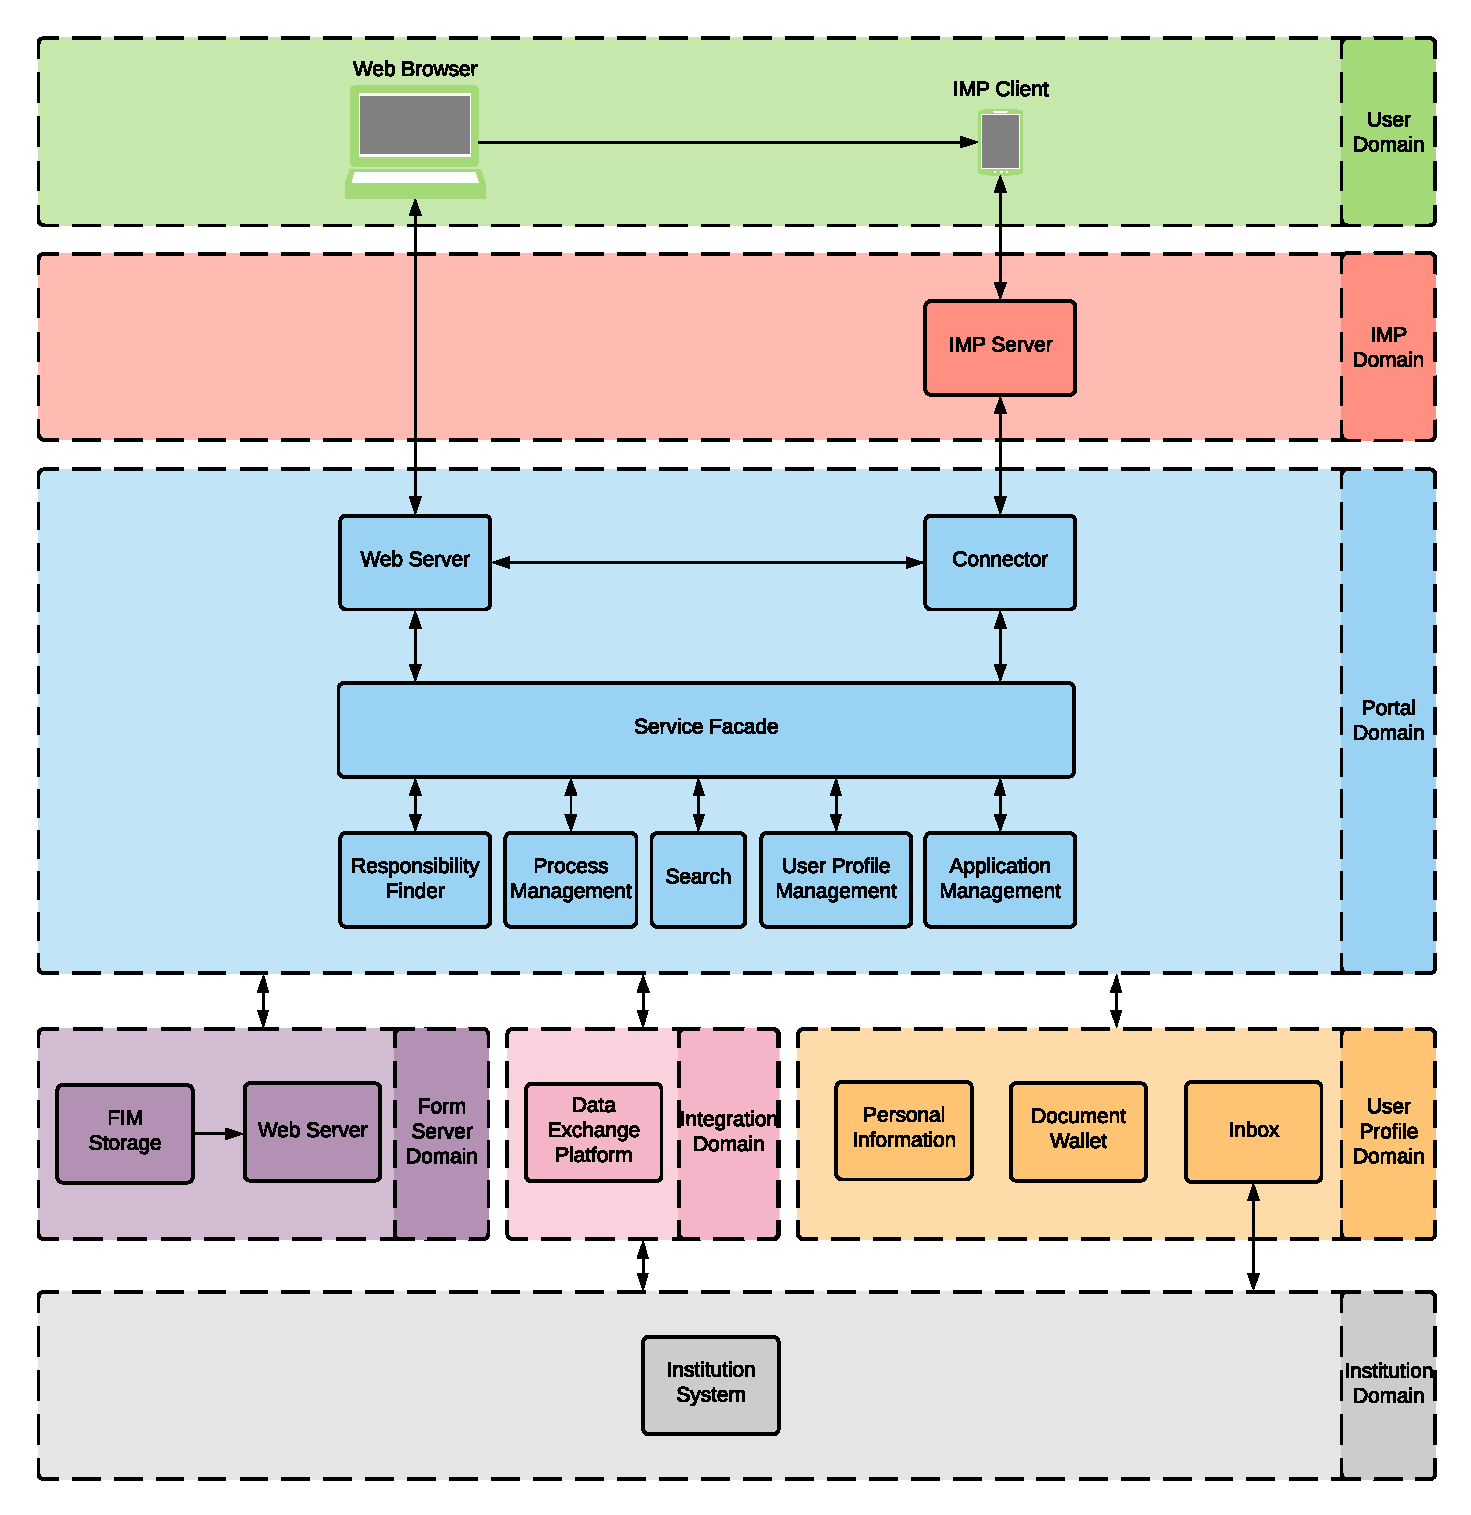
\includegraphics[scale=0.6]{Diagrams/Integration Architecture 1/Overview.pdf}
\end{center}

\begin{center}
    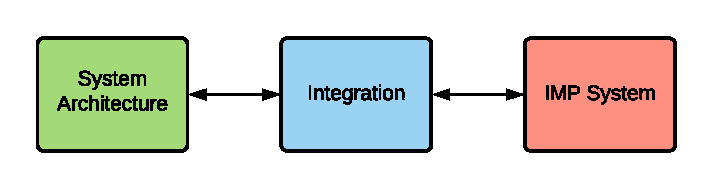
\includegraphics[scale=0.6]{Diagrams/Integration Architecture 1/Technological Integration/1. Integration Overview.pdf}
\end{center}

System architecture of the SP and IMP system consist of multiple components. The administration portal component of the system architecture is the component which will interact with the integration system. The administration portal contains a web server and a service facade. The service facade enables the administration portal amongst other things to access the user profile component. 

On the side of the IMP system, the connector will interact with the integration system.

\begin{center}
    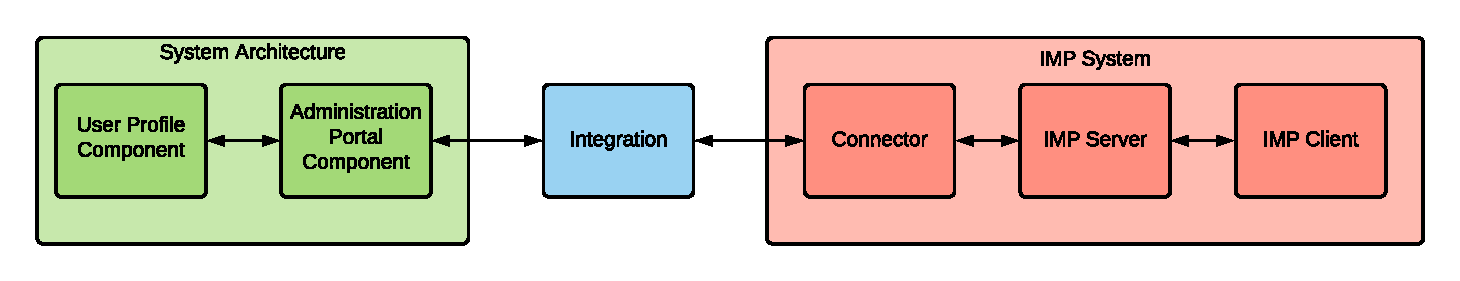
\includegraphics[scale=0.6]{Diagrams/Integration Architecture 1/Technological Integration/2. System Overview.pdf}
\end{center}

The integration is constructed as a messaging system. The messaging system consists of modules which exchange messages with connector and administration portal. As administration portal and connector are not able to send, receive or understand messages, a messaging adapter is attached to both systems. A messaging adapter is software which provides an API to the system hiding the operation of the messaging system. Depending on the system the messaging adapter should be attached to, different integration methods can be used. In most cases however, manual modification of the programming of the system is necessary to utilize the API of the adapter.

The integration system consists of messaging modules, each of them solving a different integration task. The modular approach enables the integration system to be easily expandable by new features trough new modules. Assigning integration tasks to modules also improves maintenance. System administrators can update a feature by modifying and expanding the corresponding component.
Modules can be designed to be reusable by other components which reduces the development time for new features and the size of the integration system. If the modules supports it, the performance of the integration system can be dynamically scaled by adding multiple module instances.

Modules have the purpose of solving integration tasks by providing access to features presented in section 5.1 while hiding the complexity of the operation of the IMP system. Modules therefore exchange messages through three types of publish-subscribe channels. Between administration portal and modules, feature channels are used. On these channels, messages strongly related to the operation of the system architecture of the service provider are exchanged. This are for example messages for requesting services like the transmission of a mail.

Between modules and connector, connector channels are used. These are a predetermined and limited set of channels which are used by the messaging adapter to map the functionalities of the connector to the messaging system. Messages exchanged on these channels are strongly related to the operation of the IMP system. This are for example requests and replies for relationships and templates.

Between modules, intermodule channels are used to exchange messages. Modules can exchange messages in order to access distributed functionalities of other modules.

\begin{center}
    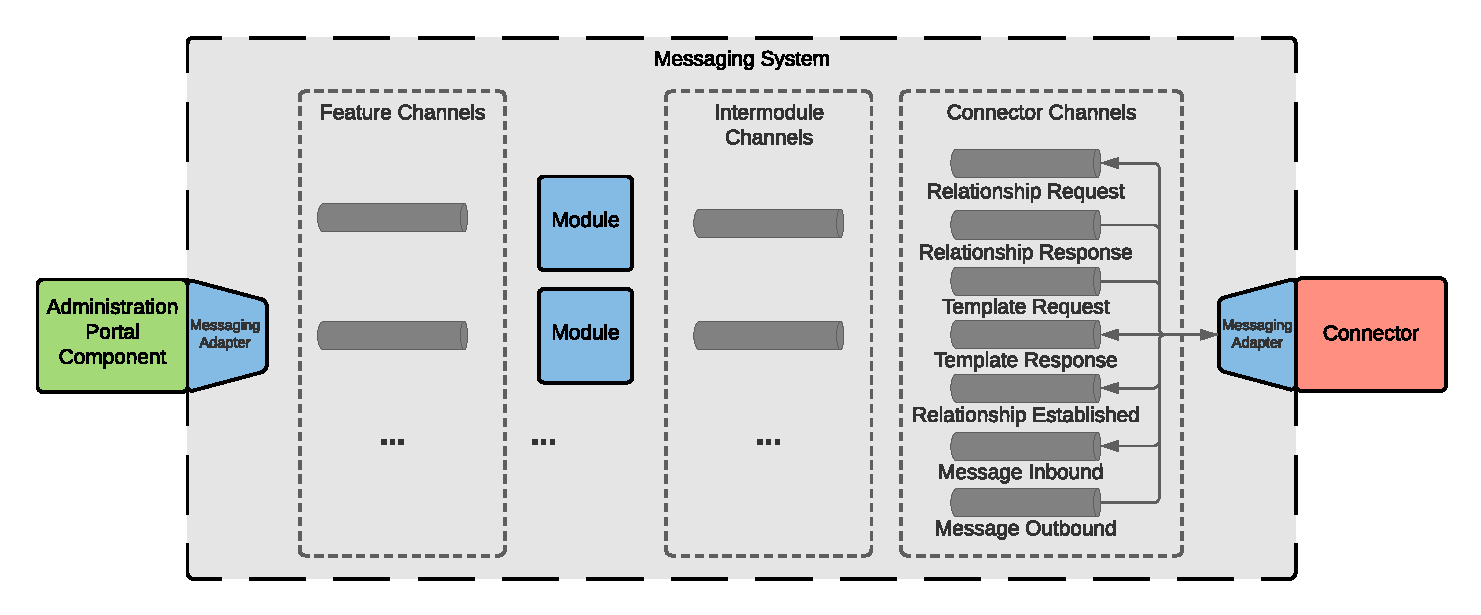
\includegraphics[scale=0.6]{Diagrams/Integration Architecture 1/Technological Integration/4. Messaging Overview.pdf}
\end{center}


As described in section 5.1, the user should be able to create a new user profile for the OZG system through an existing IMP identity.

On the existing website of the administration portal, where users can create a user profile, the relationship template for onboarding should be displayed. When the web server receives a GET request for the profile creation website, it issues a request to the messaging system for a new onboarding template. The messaging system interacts with the IMP connector to construct the template and send it back to the web server. The web server renders the template as a QR code. The QR code is displayed on the device of the user who can use the IMP client to scan it and initiate a relationship request. The messaging system interacts with the connector to establish the relationship and eventually issues the service facade to create a new user profile based on the attributes shared as part of the IMP relationship. After successful creation of the user profile, the messaging system stores the relationship ID and the user profile ID in a database. In the future, each request containing either a user profile ID or relationship ID can be mapped to the correct OZG and IMP identities. The messaging system notifies the web server of the successful creation of the user profile and the web server displays a corresponding notification to the user.

\begin{center}
    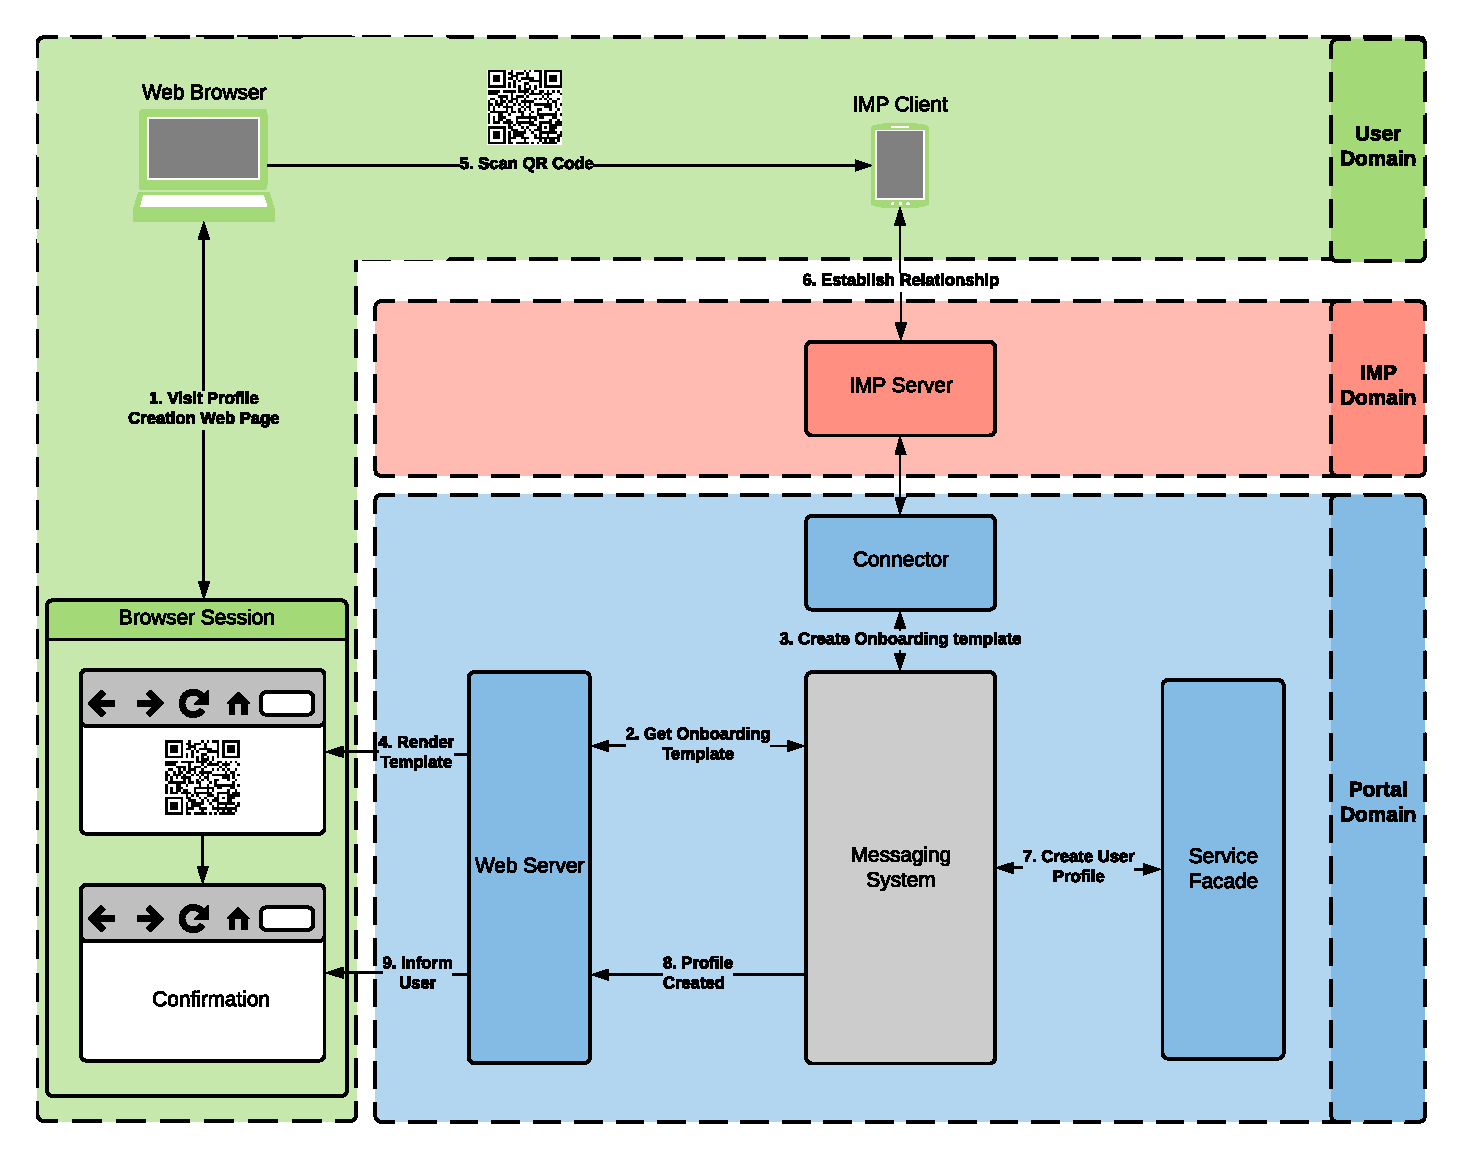
\includegraphics[scale=0.6]{Diagrams/Integration Architecture 1/Technological Integration/5. Onboarding Overview.pdf}
\end{center}

\begin{itemize}
    \item Web Server has messaging adapter with API for retrieving onboarding template
    
    \item Connector has messaging adapter with API for creating templates
    
    \item Onboarding Template Module exists, which manages the exchange of request and reply messages
    
    \item Module exchanges messages with web server adapter through request and reply channel. Only this module and the adapter of the web server use the channels.
    
    \item Module exchanges messages with connector adapter through request reply channel. Multiple different modules can use the channels. 
    
    \item Config Enricher adds suitable configuration as new entry to request
    
    \item Configuration is stored in a database or file. An administrator maintains the configuration
    
    \item The configuration creates a relationship template used to create a user profile. The configuration has to define the template to require attributes necessary for creating a user profiles.
    
    \item Attribute names and meaning can differ between OZG user profile and IMP identity, the configuration has to use the attribute definition of the IMP system.

    \item Config Message Translator incorporates the metadata entry to the template configuration
    
    \item Adapter Message Translator incorporates mapping of possible future changes of adapters in for example attribute naming or attribute data types (this type of message translator can be added to every channel connected to an adapter and is therefore excluded in future visualizations)
    
    \item Module filters for templates of the onboarding type as the channel could contain responses with templates of different type for other modules.
    
\end{itemize}


\begin{center}
    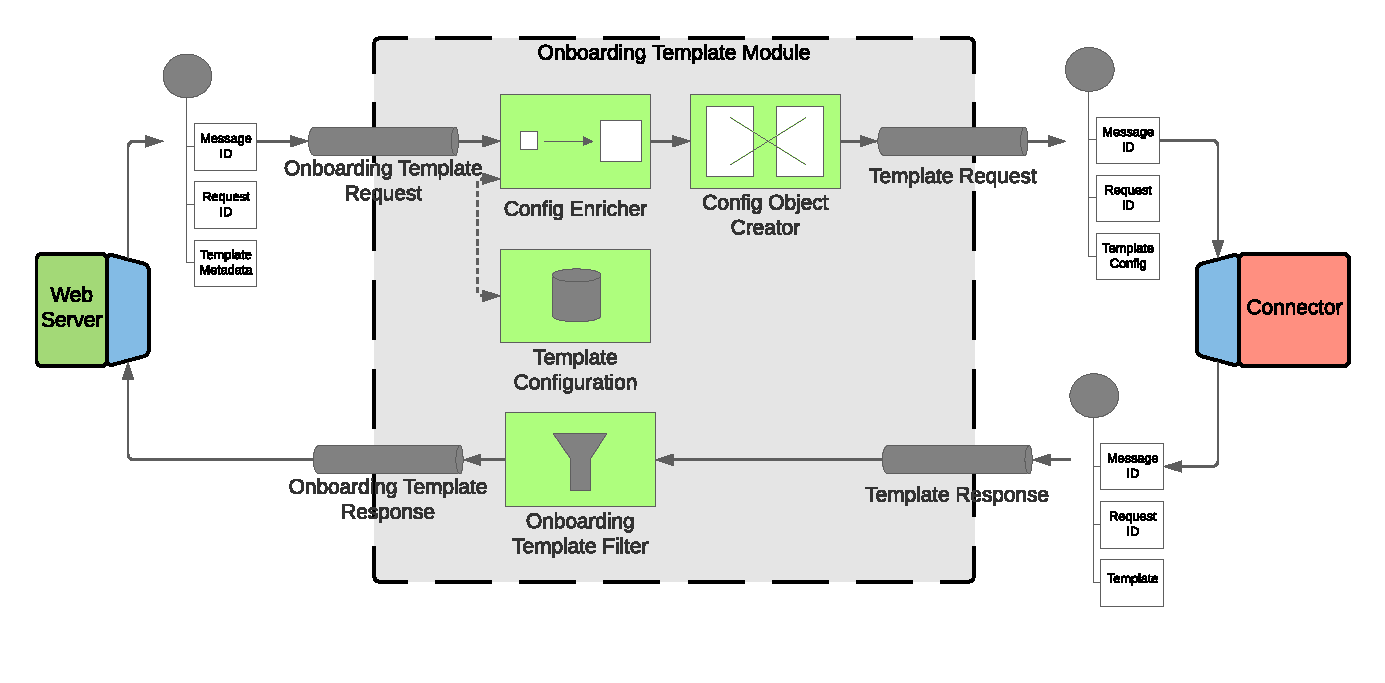
\includegraphics[scale=0.6]{Diagrams/Integration Architecture 1/Technological Integration/6. Onboarding Template Module.pdf}
\end{center}

Eventually, the user sends a relationship request which will be processed by the "Onboarding Request Module"

\begin{center}
    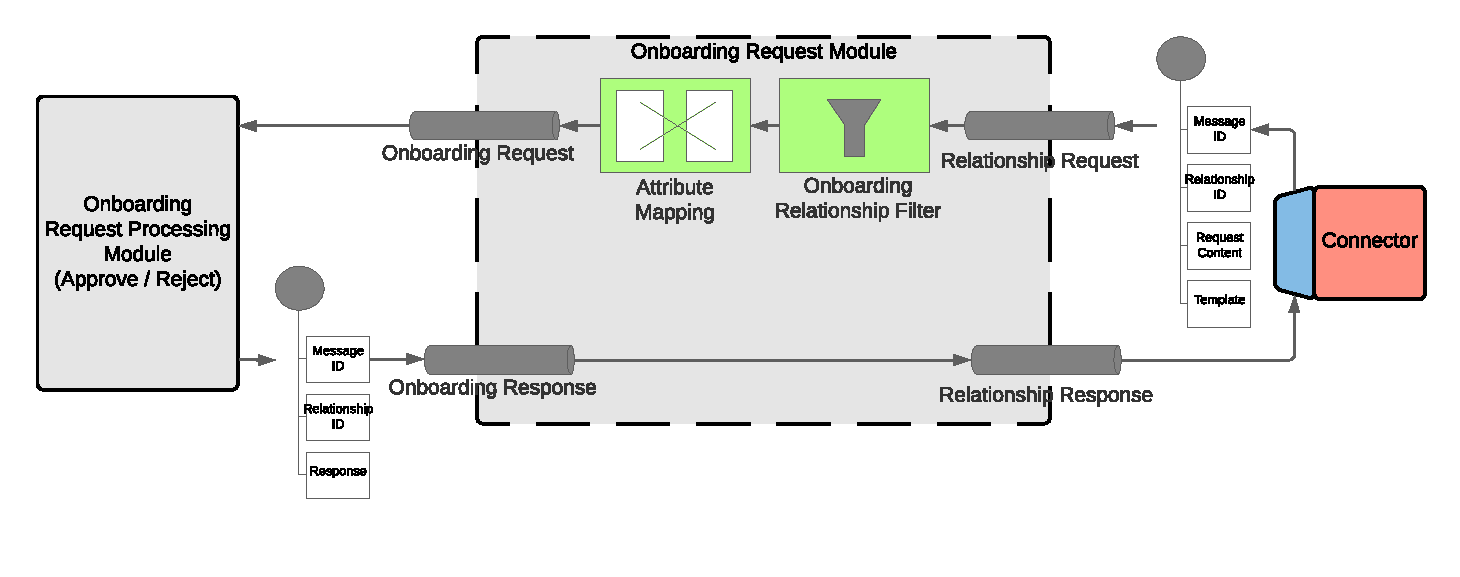
\includegraphics[scale=0.6]{Diagrams/Integration Architecture 1/Technological Integration/7. Onboarding Request Module.pdf}
\end{center}

\begin{center}
    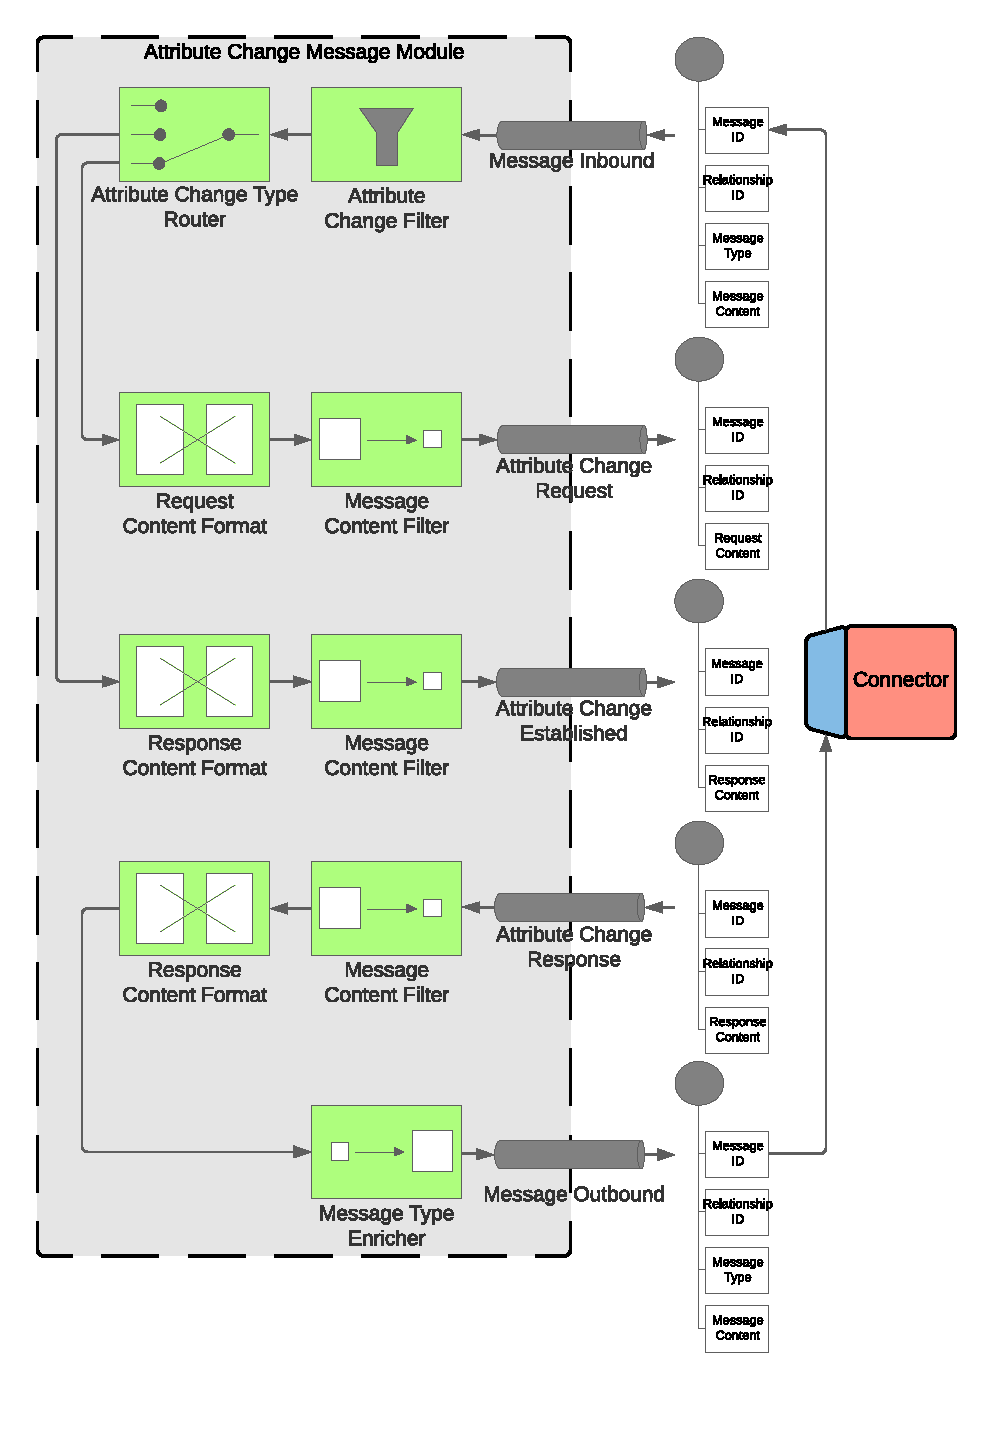
\includegraphics[scale=0.6]{Diagrams/Integration Architecture 1/Technological Integration/8. Attribute Change Message Module.pdf}
\end{center}

\begin{center}
    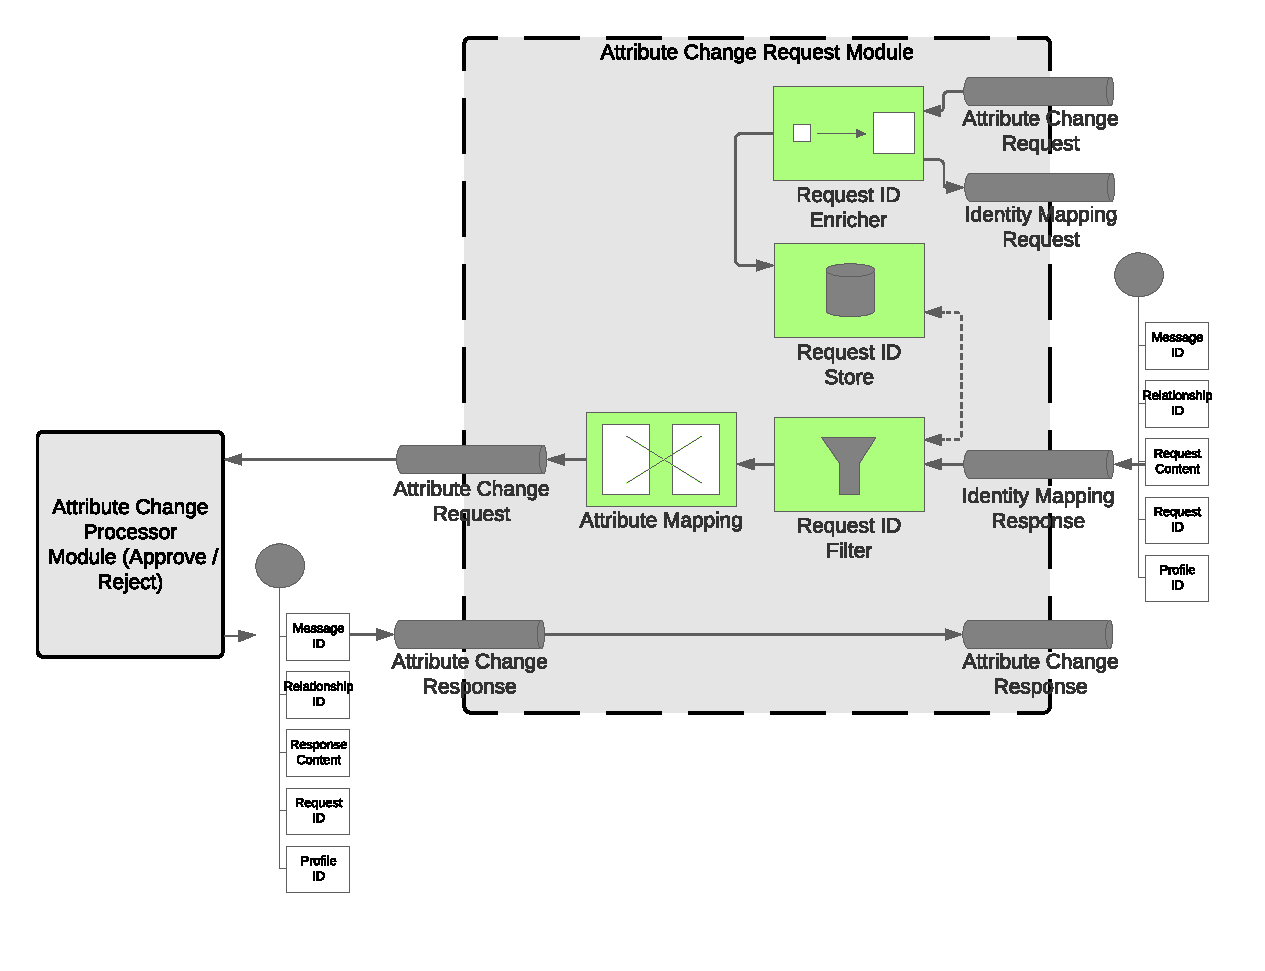
\includegraphics[scale=0.6]{Diagrams/Integration Architecture 1/Technological Integration/9. Attribute Change Request Module.pdf}
\end{center}

\begin{center}
    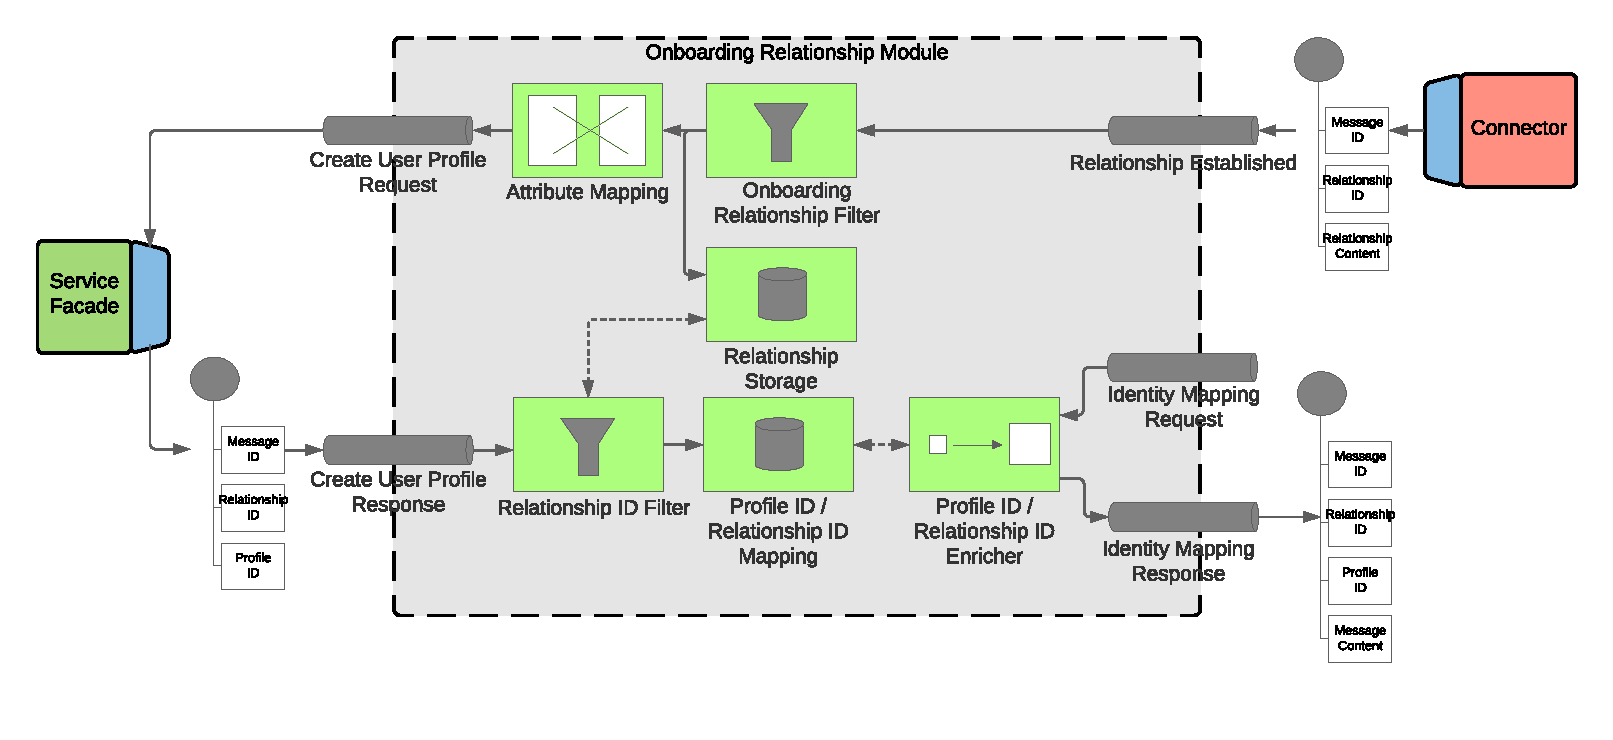
\includegraphics[scale=0.6]{Diagrams/Integration Architecture 1/Technological Integration/10. Onboarding Relationship Module.pdf}
\end{center}

\begin{center}
    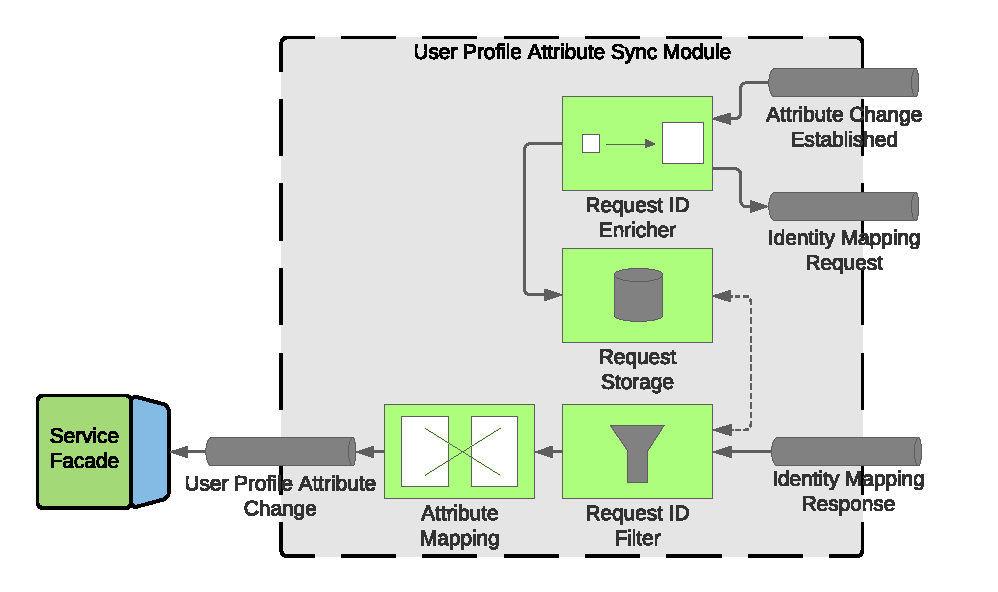
\includegraphics[scale=0.6]{Diagrams/Integration Architecture 1/Technological Integration/11. User Profile Attribute Sync Module.pdf}
\end{center}

\begin{center}
    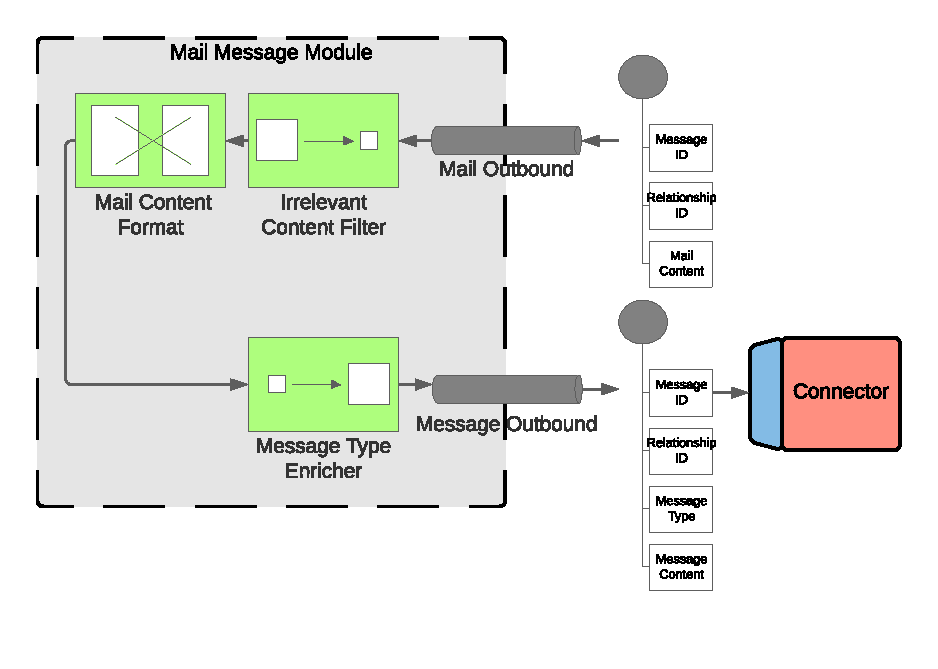
\includegraphics[scale=0.6]{Diagrams/Integration Architecture 1/Technological Integration/12. Mail Message Module.pdf}
\end{center}

\begin{center}
    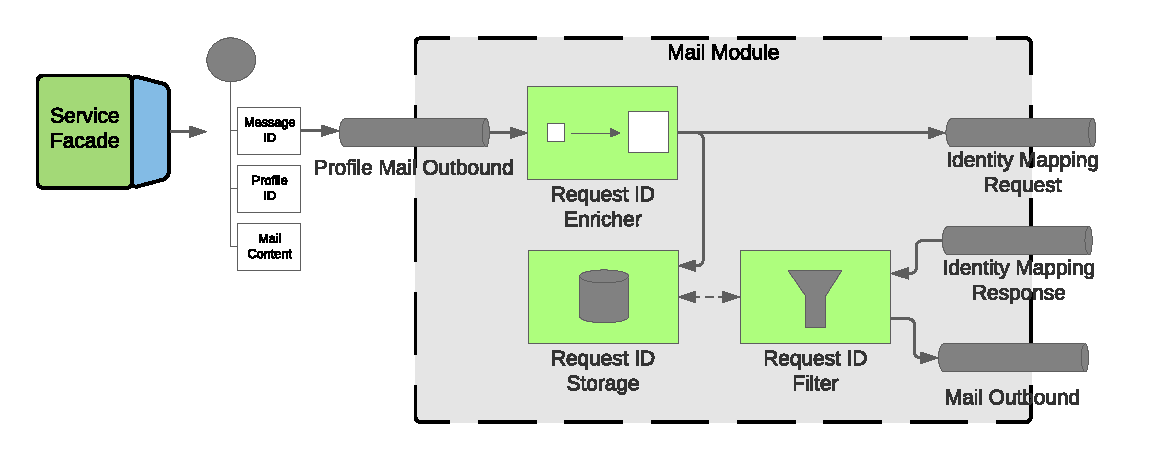
\includegraphics[scale=0.6]{Diagrams/Integration Architecture 1/Technological Integration/13. Mail Module.pdf}
\end{center}

\begin{center}
    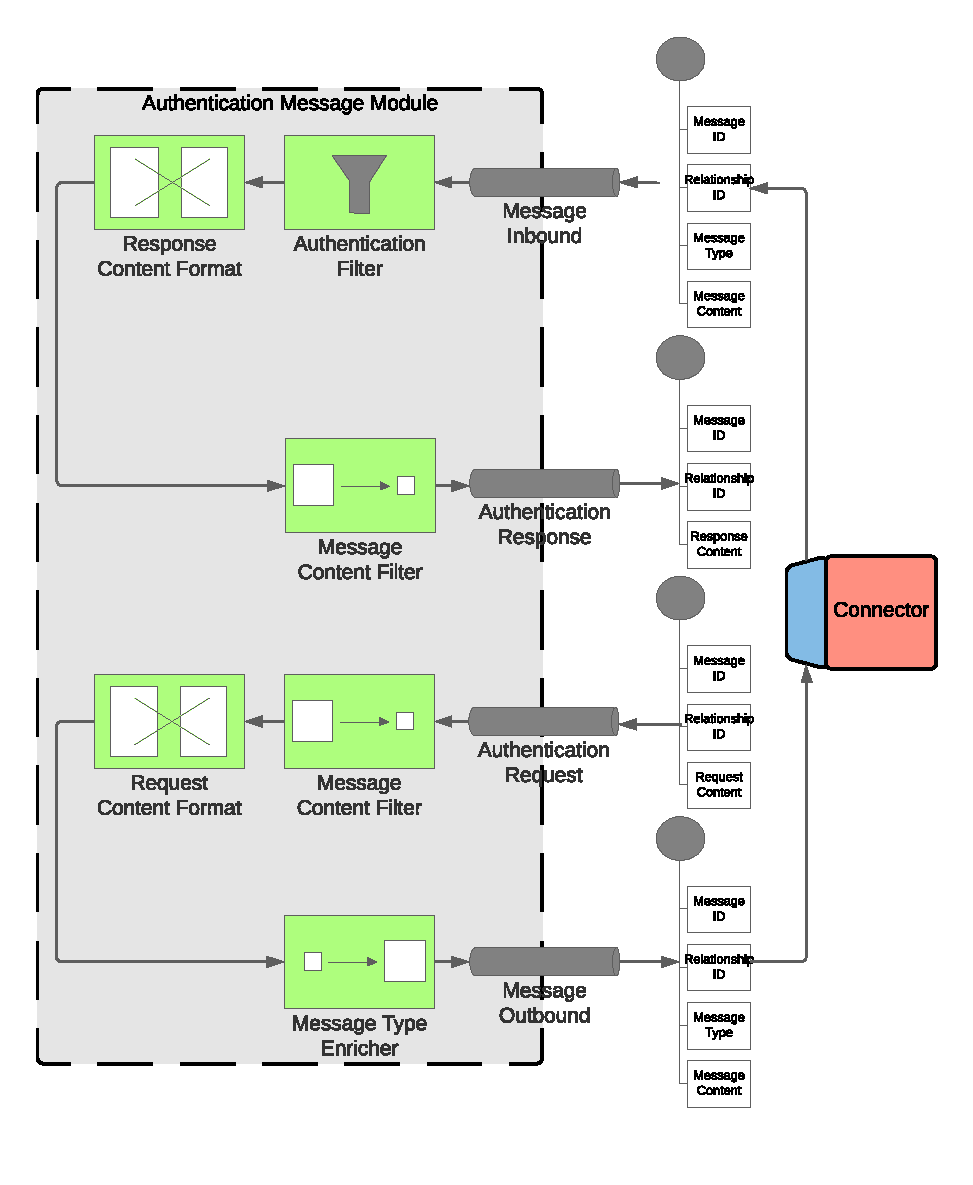
\includegraphics[scale=0.6]{Diagrams/Integration Architecture 1/Technological Integration/14. Authenticatin Message Module.pdf}
\end{center}

\begin{center}
    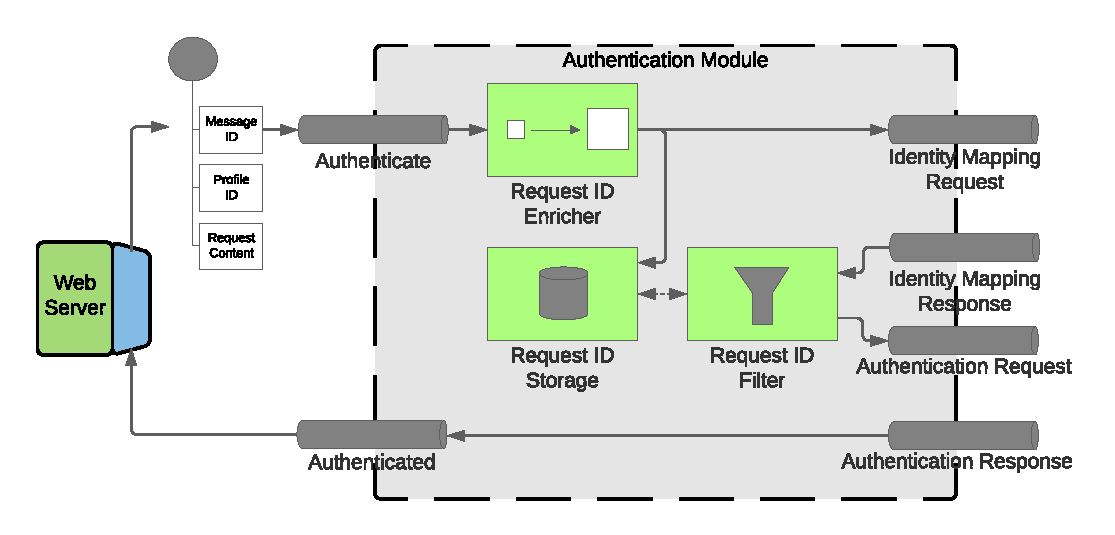
\includegraphics[scale=0.6]{Diagrams/Integration Architecture 1/Technological Integration/15. Authentication.pdf}
\end{center}